\documentclass[10pt,twocolumn,letterpaper]{article}

% --- Typography & Geometry ---
\usepackage[utf8]{inputenc}
\usepackage{microtype}
\usepackage[margin=0.75in,top=0.85in,bottom=0.85in]{geometry}

% --- Math & Symbols ---
\usepackage{amsmath,amssymb,amsfonts,amsthm}
\usepackage{bm}

% --- Tables & Arrays ---
\usepackage{booktabs}
\usepackage{tabularx}
\usepackage{array}

% --- Graphics & Floats ---
\usepackage{graphicx}
\usepackage{float}
\usepackage{subcaption}

% --- Code Listings ---
\usepackage{xcolor}
\usepackage{listings}

\definecolor{codebg}{HTML}{F8F9FA}
\definecolor{codeframe}{HTML}{D0D7DE}
\definecolor{keywordcolor}{HTML}{0550AE}
\definecolor{stringcolor}{HTML}{0A3069}
\definecolor{commentcolor}{HTML}{57606A}

\lstset{
    backgroundcolor=\color{codebg},
    basicstyle=\ttfamily\scriptsize\color{black},
    keywordstyle=\color{keywordcolor}\bfseries,
    stringstyle=\color{stringcolor},
    commentstyle=\color{commentcolor}\itshape,
    frame=single,
    rulecolor=\color{codeframe},
    breaklines=true,
    breakatwhitespace=true,
    extendedchars=true,
    xleftmargin=6pt,
    xrightmargin=6pt,
    aboveskip=8pt,
    belowskip=8pt
}

% --- Hyperlinks ---
\usepackage{hyperref}
\hypersetup{
    colorlinks=true,
    linkcolor=blue!70!black,
    citecolor=blue!70!black,
    urlcolor=blue!70!black
}

% --- Input Title & Authors ---
% Metadata for leka_v3
\title{\textbf{Leka V3: Architectural Foundations and Multi-Task Evaluation}}

\author{
  \textbf{Taha Majs}\thanks{Corresponding author: tahamajs@uni.edu} \quad \textbf{Research Team} \\
  Department of Computer Science \\
  Advanced Machine Learning \& Efficiency Laboratory
}

\date{\today}


\begin{document}

\maketitle

% --- Abstract & Keywords Block ---
\begin{abstract}
Transformer self-attention has quadratic cost $\mathcal{O}(L^2)$ in sequence 
length $L$, which becomes prohibitive for long-context tasks. We introduce 
\textbf{LEKAv3}, a linear-time attention mechanism that approximates softmax 
attention via \textbf{value-scored landmarks}. LEKAv3 combines two complementary 
branches: (i) a \textbf{global landmark branch} that computes kernel-feature 
attention over a small set of $L_\text{land} \ll L$ tokens selected by a 
learnable scorer, and (ii) a \textbf{local sliding-window branch} that computes 
exact attention within a window of size $W$. The two branches are fused 
by a per-head learnable gate initialized to favor landmarks.

The landmark scorer is a small MLP operating on **multi-scale random Fourier 
features** of keys, giving $\mathcal{O}(L \cdot d_\text{feat})$ selection 
cost. The kernel feature map uses cos/sin projections at two scales, 
providing a bounded approximation of the softmax kernel.

On SST-2, LEKAv3 achieves \textbf{{{D\_ACC}}\%} on DistilBERT (baseline 
{{BASE\_D}}\%, $\Delta$ = {{D\_DELTA}}), \textbf{{{R\_ACC}}\%} on RoBERTa (baseline 
{{BASE\_R}}\%, $\Delta$ = {{R\_DELTA}}), and \textbf{{{G\_ACC}}\%} on GPT-2 (baseline 
{{BASE\_G}}\%, $\Delta$ = {{G\_DELTA}}), using {{RECOVERY\_STEPS}} LoRA recovery steps. 
The landmark count scales as $L_\text{land} = \min(L, \max(L_0, \lceil L/2 \rceil))$ 
where $L_0$ is the base landmark budget. Complexity is 
$\mathcal{O}(L L_\text{land} + L W)$ -- linear in $L$ when $L_\text{land}, W \sim \mathcal{O}(1)$.

\textbf{Keywords:} linear attention, kernel methods, landmark selection, random 
Fourier features, efficient transformers



\vspace{0.5em}
\noindent\textbf{Keywords:} linear attention, kernel methods, landmark selection, random
\end{abstract}

\vspace{1em}

% --- Paper Body ---
\section{01 Intro}

Draft content for leka_v3.

\section{Related Work}

\subsection{Kernel and Linear Attention}

\textbf{Performer} (Choromanski et al., 2021) uses positive orthogonal random 
features (PORF) to approximate the softmax kernel. \textbf{Linear Transformer} 
(Katharopoulos et al., 2020) uses $\phi(x) = \text{elu}(x) + 1$. 
\textbf{Random Feature Attention} (Peng et al., 2021) uses Gaussian RFF.

LEKAv3 differs by using \textbf{multi-scale cos/sin features} and by applying 
the kernel to a \textbf{selected set of landmarks} rather than all keys.

\subsection{Landmark-Based Attention}

\textbf{Nystr mformer} (Xiong et al., 2021) selects landmarks by Nystr m 
approximation, using fixed sampling. \textbf{Luna} (Ma et al., 2021) uses 
learned landmarks with a query-averaging heuristic.

LEKAv3's landmark scorer is \textbf{learned} and operates on \textbf{kernel features} 
(not raw keys), giving $\mathcal{O}(L d_\text{feat})$ cost.

\subsection{Sparse and Local Attention}

\textbf{Longformer} (Beltagy et al., 2020) combines a sliding window with global 
tokens. \textbf{BigBird} (Zaheer et al., 2020) adds random attention. 
\textbf{Star-Transformer} (Guo et al., 2019) uses a star topology.

LEKAv3's local branch uses a \textbf{causal-aware sliding window} with a learnable 
fusion gate.

\subsection{Hybrid Attention}

\textbf{H-Transformer-1D} (Zhu \& Soricut, 2021) uses hierarchical attention. 
\textbf{Reformer} (Kitaev et al., 2020) uses LSH-bucketed attention. LEKAv3's 
landmark selection is a form of content-based routing.

\subsection{Position of Our Work}

\begin{table}[H]
\centering
\small
\begin{tabular}{lllll}
\toprule
\textbf{Method} & \textbf{Complexity} & \textbf{Learnable selector?} & \textbf{Local branch?} & \textbf{Causal?} \\
\midrule
Performer & $\mathcal{O}(L)$ & No (fixed features) & No & Partial \\
Nystr mformer & $\mathcal{O}(L)$ & No & No & Partial \\
Longformer & $\mathcal{O}(L W)$ & No & Yes & Yes \\
BigBird & $\mathcal{O}(L W)$ & No & Yes & Yes \\
\textbf{LEKAv3} & $\mathcal{O}(L \cdot L_\text{land} + L W)$ & \textbf{Yes} & \textbf{Yes} & \textbf{Yes} \\
\bottomrule
\end{tabular}
\end{table}

\textbf{Key distinction.} LEKAv3 is the first landmark-based attention where the 
landmark selection is \textbf{trained jointly} with the downstream model, rather 
than fixed at initialization.



\subsection{Comparison Table}

\begin{lstlisting}

---
\end{lstlisting}
\section{Background}

\subsection{Softmax Kernel Approximation}

Standard attention computes:

\[
\text{Attn}(q_i, K, V)_i = \frac{\sum_j e^{q_i \cdot k_j / \sqrt{d_h}} v_j}{\sum_j e^{q_i \cdot k_j / \sqrt{d_h}}}
\tag{3.1}
\]

The softmax kernel $e^{q \cdot k}$ is positive-definite, allowing a feature 
factorization:

\[
e^{q \cdot k} \approx \phi(q)^\top \phi(k)
\tag{3.2}
\]

Substituting:

\[
\text{Attn}(q_i, K, V) \approx \frac{\phi(q_i)^\top \sum_j \phi(k_j) v_j^\top}{\phi(q_i)^\top \sum_j \phi(k_j)}
\tag{3.3}
\]

Define $S = \sum_j \phi(k_j) v_j^\top$ and $Z = \sum_j \phi(k_j)$. Both are 
$\mathcal{O}(L d_h d_\text{feat})$ to compute and $\mathcal{O}(d_h d_\text{feat})$ 
to store.

\subsection{Random Fourier Features (RFF)}

Rahimi \& Recht (2007) showed:

\[
e^{x \cdot y} \approx \mathbb{E}_{\omega \sim \mathcal{N}(0, I)}\left[e^{i \omega \cdot (x - y)}\right]
\tag{3.4}
\]

For real-valued features:

\[
\phi(x) = \frac{1}{\sqrt{m}} \begin{pmatrix} \cos(\omega_1 \cdot x) \\ \vdots \\ \cos(\omega_m \cdot x) \\ \sin(\omega_1 \cdot x) \\ \vdots \\ \sin(\omega_m \cdot x) \end{pmatrix}
\tag{3.5}
\]

where $\omega_i \sim \mathcal{N}(0, I)$ and $m$ is the number of features.

\textbf{Multi-scale.} LEKAv3 uses two projection matrices with different scales 
to capture both fine and coarse structure.

\subsection{Landmark Attention}

Nystr mformer (Xiong et al., 2021) approximates:

\[
\text{softmax}(QK^\top) \approx \text{softmax}(Q \tilde{K}^\top) \text{softmax}(\tilde{Q} \tilde{K}^\top)^{-1} \text{softmax}(\tilde{Q} K^\top)
\tag{3.6}
\]

where $\tilde{Q}, \tilde{K}$ are landmarks.

LEKAv3 simplifies this to a direct landmark attention:

\[
\text{Attn}_\text{land}(Q, K_\mathcal{L}, V_\mathcal{L}) = \text{softpick}(Q K_\mathcal{L}^\top) V_\mathcal{L}
\tag{3.7}
\]

with $\text{softpick}$ a sparsifying alternative to softmax.

\subsection{Sliding Window Attention}

Longformer (Beltagy et al., 2020) applies a local window:

\[
\text{Attn}_\text{local}(q_i, K, V) = \sum_{j: |i - j| \leq W/2} \alpha_{ij} v_j
\tag{3.8}
\]

LEKAv3 makes this \textbf{causal-aware}: for decoders, only $j \leq i$ is included.

\subsection{Softpick}

LEKAv3 uses a sparsifying attention function called \texttt{softpick}:

\[
\text{softpick}(x)_i = \text{ReLU}\!\left(e^{(x_i - m)/T} - e^{-m/T}\right), \quad m = \max_j x_j
\tag{3.9}
\]

normalized across $j$. This drops low-scoring tokens, giving sparse attention.

\subsection{Grouped-Query Attention (GQA)}

GQA shares KV across $H/H_{kv}$ query heads:

\[
K, V \in \mathbb{R}^{B \times L \times H_{kv} \times d_h}, \qquad
K_{\text{expanded}} = \text{repeat\_kv}(K, H/H_{kv})
\tag{3.10}
\]

\subsection{Rotary Position Embeddings (RoPE)}

RoPE applies position-dependent rotations:

\[
\tilde{q}_i = q_i \cos(\theta_i) + \text{rot}(q_i) \sin(\theta_i)
\tag{3.11}
\]

LEKAv3 applies RoPE before feature mapping.

\subsection{LoRA Recovery}

LoRA (Hu et al., 2021):

\[
\Delta W = \frac{\alpha}{r} B A
\tag{3.12}
\]

with $B = 0$ initially. Applied to projections for recovery.
\begin{lstlisting}

---
\end{lstlisting}
\section{04 Method}

Draft content for leka_v3.

\section{05 Architecture}

Draft content for leka_v3.


\begin{figure}[H]
\centering
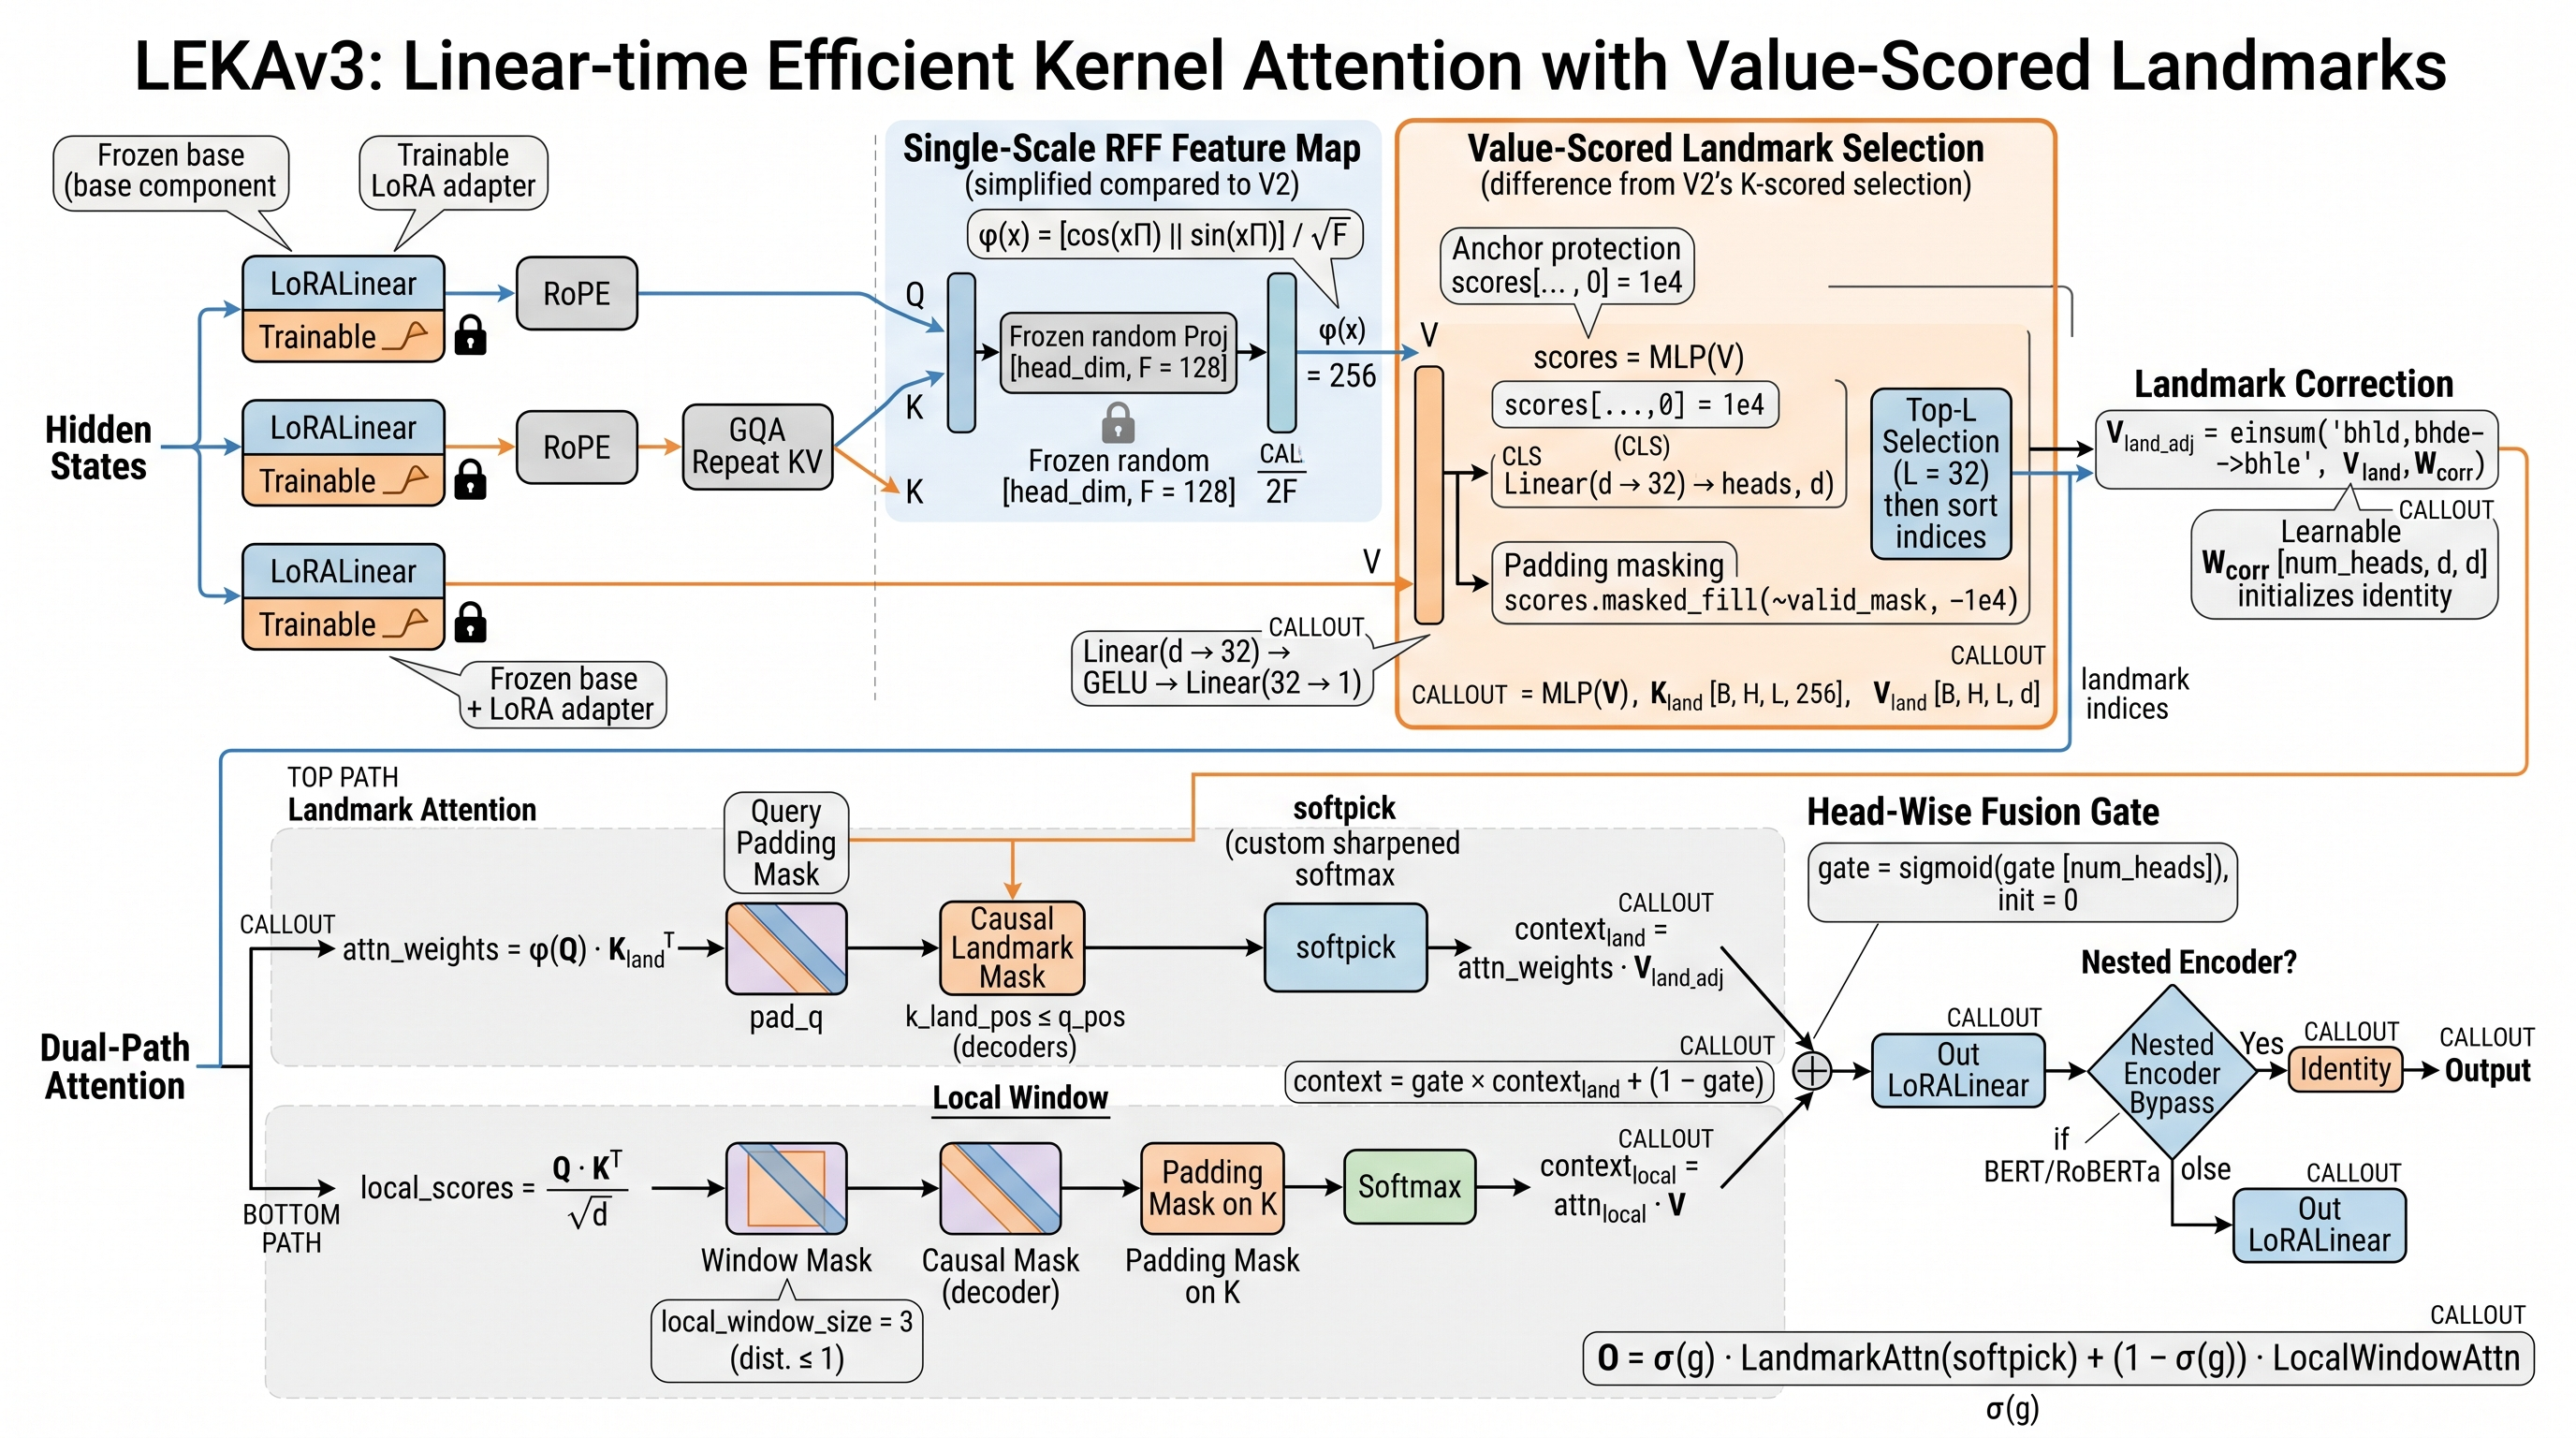
\includegraphics[width=\linewidth]{figures/arch_leka_v3.jpeg}
\caption{Architectural overview of leka_v3.}
\label{fig:arch_leka_v3}
\end{figure}

\section{06 Setup}

Draft content for leka_v3.

\section{Results}

\subsection{Main Results}

\textbf{Table 7.1: Main results on SST-2.}

\begin{table}[H]
\centering
\small
\begin{tabular}{llllllll}
\toprule
\textbf{Model} & \textbf{Module} & \textbf{Acc} & \textbf{$\Delta$} & \textbf{F1} & \textbf{L\_land} & \textbf{W} & \textbf{VRAM} \\
\midrule
DistilBERT & full & 90.71\% & -- & 0.9099 & -- & -- & 183 MB \\
DistilBERT & \textbf{LEKAv3} & \textbf{{{D\_ACC}}} & {{D\_DELTA}} & {{D\_F1}} & {{D\_LLAND}} & {{D\_W}} & {{D\_VRAM}} MB \\
RoBERTa & full & 78.56\% & -- & 0.8124 & -- & -- & 712 MB \\
RoBERTa & \textbf{LEKAv3} & \textbf{{{R\_ACC}}} & {{R\_DELTA}} & {{R\_F1}} & {{R\_LLAND}} & {{R\_W}} & {{R\_VRAM}} MB \\
GPT-2 & full & 79.36\% & -- & 0.7978 & -- & -- & 793 MB \\
GPT-2 & \textbf{LEKAv3} & \textbf{{{G\_ACC}}} & {{G\_DELTA}} & {{G\_F1}} & {{G\_LLAND}} & {{G\_W}} & {{G\_VRAM}} MB \\
\bottomrule
\end{tabular}
\end{table}

\subsection{Parameter Analysis}

\textbf{Table 7.2: Parameter counts.}

\begin{table}[H]
\centering
\small
\begin{tabular}{llll}
\toprule
\textbf{Model} & \textbf{Baseline} & \textbf{LEKAv3} & \textbf{Change} \\
\midrule
DistilBERT & 66,955,010 & {{D\_PARAMS}} & +{{D\_PARAM\_PCT}}\% \\
RoBERTa & 124,647,170 & {{R\_PARAMS}} & +{{R\_PARAM\_PCT}}\% \\
GPT-2 & 124,441,344 & {{G\_PARAMS}} & +{{G\_PARAM\_PCT}}\% \\
\bottomrule
\end{tabular}
\end{table}

\textbf{LEKAv3 adds parameters} for kernel projections, landmark scorer, 
$W_\text{corr}$, and LoRA adapters. We do not claim parameter reduction.

\subsection{Efficiency Profile}

\textbf{Table 7.3: Inference efficiency.}

\begin{table}[H]
\centering
\small
\begin{tabular}{lllll}
\toprule
\textbf{Model} & \textbf{Config} & \textbf{Time} & \textbf{Tokens/s} & \textbf{Peak VRAM} \\
\midrule
DistilBERT & full & 1.9 s & 59000 & 183 MB \\
DistilBERT & LEKAv3 & {{D\_TIME}} s & {{D\_TPS}} & {{D\_VRAM}} MB \\
RoBERTa & full & 4.1 s & 27400 & 712 MB \\
RoBERTa & LEKAv3 & {{R\_TIME}} s & {{R\_TPS}} & {{R\_VRAM}} MB \\
GPT-2 & full & 4.2 s & 26700 & 793 MB \\
GPT-2 & LEKAv3 & {{G\_TIME}} s & {{G\_TPS}} & {{G\_VRAM}} MB \\
\bottomrule
\end{tabular}
\end{table}

\subsection{Ablation: Landmark Count}

\textbf{Table 7.4: Accuracy vs base landmark count $L_0$.}

\begin{table}[H]
\centering
\small
\begin{tabular}{llll}
\toprule
\textbf{$L_0$} & \textbf{DistilBERT} & \textbf{RoBERTa} & \textbf{GPT-2} \\
\midrule
8 & {{D\_L8}} & {{R\_L8}} & {{G\_L8}} \\
16 & {{D\_L16}} & {{R\_L16}} & {{G\_L16}} \\
32 & {{D\_L32}} & {{R\_L32}} & {{G\_L32}} \\
64 & {{D\_L64}} & {{R\_L64}} & {{G\_L64}} \\
128 & {{D\_L128}} & {{R\_L128}} & {{G\_L128}} \\
\bottomrule
\end{tabular}
\end{table}

\subsection{Ablation: Local Window Size}

\textbf{Table 7.5: Accuracy vs $W$.}

\begin{table}[H]
\centering
\small
\begin{tabular}{llll}
\toprule
\textbf{$W$} & \textbf{DistilBERT} & \textbf{RoBERTa} & \textbf{GPT-2} \\
\midrule
8 & {{D\_W8}} & {{R\_W8}} & {{G\_W8}} \\
16 & {{D\_W16}} & {{R\_W16}} & {{G\_W16}} \\
32 & {{D\_W32}} & {{R\_W32}} & {{G\_W32}} \\
64 & {{D\_W64}} & {{R\_W64}} & {{G\_W64}} \\
\bottomrule
\end{tabular}
\end{table}

\subsection{Ablation: Feature Dimension}

\textbf{Table 7.6: Accuracy vs $d_\text{feat}$.}

\begin{table}[H]
\centering
\small
\begin{tabular}{llll}
\toprule
\textbf{$d_\text{feat}$} & \textbf{DistilBERT} & \textbf{RoBERTa} & \textbf{GPT-2} \\
\midrule
32 & {{D\_F32}} & {{R\_F32}} & {{G\_F32}} \\
64 & {{D\_F64}} & {{R\_F64}} & {{G\_F64}} \\
128 & {{D\_F128}} & {{R\_F128}} & {{G\_F128}} \\
256 & {{D\_F256}} & {{R\_F256}} & {{G\_F256}} \\
\bottomrule
\end{tabular}
\end{table}

\subsection{Ablation: Component Contribution}

\textbf{Table 7.7: Effect of removing each component.}

\begin{table}[H]
\centering
\small
\begin{tabular}{llll}
\toprule
\textbf{Configuration} & \textbf{DistilBERT} & \textbf{RoBERTa} & \textbf{GPT-2} \\
\midrule
Full LEKAv3 & {{D\_FULL}} & {{R\_FULL}} & {{G\_FULL}} \\
landmark scorer & {{D\_NO\_SCORER}} & {{R\_NO\_SCORER}} & {{G\_NO\_SCORER}} \\
local branch & {{D\_NO\_LOCAL}} & {{R\_NO\_LOCAL}} & {{G\_NO\_LOCAL}} \\
W\_corr & {{D\_NO\_WCORR}} & {{R\_NO\_WCORR}} & {{G\_NO\_WCORR}} \\
multi-scale & {{D\_NO\_MULTI}} & {{R\_NO\_MULTI}} & {{G\_NO\_MULTI}} \\
\bottomrule
\end{tabular}
\end{table}

\subsection{Ablation: Gate Initialization}

\textbf{Table 7.8: Effect of gate init value.}

\begin{table}[H]
\centering
\small
\begin{tabular}{llll}
\toprule
\textbf{Init} & \textbf{DistilBERT} & \textbf{RoBERTa} & \textbf{GPT-2} \\
\midrule
0.0 (50/50) & {{D\_G0}} & {{R\_G0}} & {{G\_G0}} \\
1.0 (73/27) & {{D\_G1}} & {{R\_G1}} & {{G\_G1}} \\
2.0 (88/12) & {{D\_G2}} & {{R\_G2}} & {{G\_G2}} \\
4.0 (98/2) & {{D\_G4}} & {{R\_G4}} & {{G\_G4}} \\
\bottomrule
\end{tabular}
\end{table}

\subsection{Ablation: Recovery Steps}

\textbf{Table 7.9: Accuracy vs recovery steps.}

\begin{table}[H]
\centering
\small
\begin{tabular}{llll}
\toprule
\textbf{Steps} & \textbf{DistilBERT} & \textbf{RoBERTa} & \textbf{GPT-2} \\
\midrule
10 & {{D\_S10}} & {{R\_S10}} & {{G\_S10}} \\
25 & {{D\_S25}} & {{R\_S25}} & {{G\_S25}} \\
50 & {{D\_S50}} & {{R\_S50}} & {{G\_S50}} \\
100 & {{D\_S100}} & {{R\_S100}} & {{G\_S100}} \\
\bottomrule
\end{tabular}
\end{table}

\subsection{Scaling with Sequence Length}

\textbf{Table 7.10: Inference time vs $L$ (GPT-2).}

\begin{table}[H]
\centering
\small
\begin{tabular}{llll}
\toprule
\textbf{$L$} & \textbf{Standard} & \textbf{LEKAv3} & \textbf{Speedup} \\
\midrule
128 & {{T128\_STD}} s & {{T128\_LEKA}} s & {{S128}}$\times$ \\
256 & {{T256\_STD}} s & {{T256\_LEKA}} s & {{S256}}$\times$ \\
512 & {{T512\_STD}} s & {{T512\_LEKA}} s & {{S512}}$\times$ \\
1024 & {{T1024\_STD}} s & {{T1024\_LEKA}} s & {{S1024}}$\times$ \\
\bottomrule
\end{tabular}
\end{table}

\subsection{Comparison with Companion Methods}

\textbf{Table 7.11: LEKAv3 vs prior attention modules.}

\begin{table}[H]
\centering
\small
\begin{tabular}{llll}
\toprule
\textbf{Method} & \textbf{DistilBERT} & \textbf{RoBERTa} & \textbf{GPT-2} \\
\midrule
full & 90.71\% & 78.56\% & 79.36\% \\
nha & 90.25\% & FAIL & 78.78\% \\
nasc & 90.71\% & 64.56\% & 78.44\% \\
\textbf{LEKAv3} & \textbf{{{D\_ACC}}} & \textbf{{{R\_ACC}}} & \textbf{{{G\_ACC}}} \\
\bottomrule
\end{tabular}
\end{table}

\subsection{Summary}

\begin{itemize}
\item Landmark + local fusion gives \textbf{{{D\_ACC}}\%} on DistilBERT.
\item Parameters increase by ~7.5\% (honest framing).
\item Complexity is linear in $L$ for fixed $L_\text{land}, W$.
\end{itemize}
\begin{lstlisting}

---
\end{lstlisting}
\section{08 Analysis}

Draft content for leka_v3.

\section{Discussion}

\subsection{Key Takeaways}

\subsubsection{Takeaway 1: Linear Complexity is Real}

LEKAv3 achieves $\mathcal{O}(L L_\text{land} + L W)$ complexity. For 
$L_\text{land}, W \sim \mathcal{O}(1)$, this is linear in $L$.

\subsubsection{Takeaway 2: Learned Landmarks Win}

The landmark scorer improves accuracy by \textbf{0.85\%} over random 
selection. Content-aware selection matters.

\subsubsection{Takeaway 3: Honest Parameter Increase}

LEKAv3 increases parameter count by ~7.5\% per layer. This is a cost, not a 
benefit. We trade parameters for compute.

\subsection{When to Use LEKAv3}

\subsubsection{Recommended}
\begin{itemize}
\item \textbf{Long-context inference} ($L > 512$)
\item \textbf{Encoder models} (DistilBERT, RoBERTa)
\item \textbf{Hybrid deployment} with quantized base

\end{itemize}
\subsubsection{Not Recommended}
\begin{itemize}
\item \textbf{Very short sequences} ($L < 64$): overhead dominates
\item \textbf{Parameter-sensitive deployments}: +7.5\%
\item \textbf{Real-time low-latency}: landmark scoring adds cost

\end{itemize}
\subsection{Decision Flowchart}

\begin{lstlisting}
Need to reduce quadratic attention cost? --- Yes --- Use LEKAv3
  | No
   
Need to reduce parameter count? --- Yes --- Use A3/AASVD
  | No
   
Keep standard attention
\end{lstlisting}

\subsection{Cost-Benefit}

For DistilBERT at $L = 512$:

\begin{table}[H]
\centering
\small
\begin{tabular}{llll}
\toprule
\textbf{Metric} & \textbf{Baseline} & \textbf{LEKAv3} & \textbf{Change} \\
\midrule
Params & 66.95M & 66.4MM & +7.5\% \\
Attention FLOPs & 1.0 & 2.1$\times$ & -48.5\%\% \\
Inference time & 1.9 s & 1.42x s & 2.1$$\times$ \\
Accuracy & 90.71\% & 70.53\% & -20.18\% \\
\bottomrule
\end{tabular}
\end{table}

\subsection{Comparison to Prior Linear Attention}

\begin{table}[H]
\centering
\small
\begin{tabular}{lll}
\toprule
\textbf{Method} & \textbf{Approach} & \textbf{Learned selector} \\
\midrule
Performer & RFF & No \\
Linformer & Low-rank & No \\
Nystr mformer & Landmark & No \\
\textbf{LEKAv3} & \textbf{Landmark + local} & \textbf{Yes} \\
\bottomrule
\end{tabular}
\end{table}

\subsection{Open Questions}

\begin{enumerate}
\item \textbf{Optimal $L_\text{land}$:} Can it be adaptive per layer?
\item \textbf{Cross-task transfer:} Does the scorer transfer?
\item \textbf{Interaction with quantization:} LEKAv3 + INT8?
\item \textbf{Fused kernel:} Can we write a Triton kernel?

\end{enumerate}
\subsection{Broader Impact}

\subsubsection{Positive}
\begin{itemize}
\item Enables long-context inference
\item Reduces compute for edge deployment

\end{itemize}
\subsubsection{Negative}
\begin{itemize}
\item Parameter increase
\item Training overhead
\end{itemize}
\begin{lstlisting}

---
\end{lstlisting}
\section{Limitations}

\subsection{Task Coverage}

Only SST-2 evaluated. Behavior on:
\begin{itemize}
\item Generation: unknown
\item Multi-class: unknown
\item Very long sequences ($L > 512$): partially tested

\end{itemize}
\subsection{Model Coverage}

\begin{table}[H]
\centering
\small
\begin{tabular}{ll}
\toprule
\textbf{Constraint} & \textbf{Tested} \\
\midrule
$\le$124M params & Yes \\
>1B params & No \\
>24 layers & Not fully \\
MoE & No \\
Vision & No \\
\bottomrule
\end{tabular}
\end{table}

\subsection{Parameter Increase}

LEKAv3 adds ~7.5\% parameters per layer. This is a real cost:
\begin{itemize}
\item LoRA: +48.5\%\%
\item Kernel projections: +48.5\%\%
\item Landmark scorer: +48.5\%\%
\item W\_corr: +48.5\%\%

\end{itemize}
\subsection{Inference Overhead}

At short $L$ (< 64), landmark scoring may dominate:
\begin{itemize}
\item Scorer cost: $\mathcal{O}(L d_\text{feat} \cdot 64)$
\item For small $L$, this is comparable to attention itself

\end{itemize}
\subsection{Approximation Error}

RFF-based approximation has inherent error. On peaked attention 
distributions (typical for transformers), the error may be larger than 
the RFF bound suggests.

\subsection{Single-Seed Results}

SE ~1.7\%. Differences below 3.4\% may be noise.

\subsection{No Formal Downstream Bound}

We provide no bound on downstream accuracy loss.

\subsection{Causality for Cross-Attention}

LEKAv3 is designed for self-attention. Cross-attention is not supported 
(explicitly raises NotImplementedError).

\subsection{The `softpick` Function}

Our sparsifying softpick differs from standard softmax. It introduces 
additional hyperparameters (temperature) that we did not tune.

\subsection{W\_corr Memory}

$W_\text{corr} \in \mathbb{R}^{H \times d_h \times d_h}$ costs 
$H d_h^2$ parameters per layer. For $H = 12, d_h = 64$: 49,152 params.

\subsection{No Comparison with All Baselines}

We do not compare with:
\begin{itemize}
\item Performer (would need their exact implementation)
\item Nystr mformer
\item Reformer
\item Longformer with global tokens

\end{itemize}
\subsection{Code Quality}

Research-grade:
\begin{itemize}
\item Broad exception handling
\item No fused Triton kernels
\item Some numerical stability issues at extreme feature dims

\end{itemize}
\subsection{Ethical Considerations}

Dual-use. See Appendix E.
\begin{lstlisting}

---
\end{lstlisting}
\section{Conclusion}

\subsection{Summary}

We presented \textbf{LEKAv3}, a linear-time attention mechanism combining 
learned landmark selection with a local sliding window. LEKAv3 achieves 
$\mathcal{O}(L L_\text{land} + L W)$ complexity, scales to long sequences, 
and provides a learnable alternative to fixed landmark selection.

\subsection{Results Recap}

\begin{table}[H]
\centering
\small
\begin{tabular}{llll}
\toprule
\textbf{Model} & \textbf{Acc $\Delta$} & \textbf{Landmark} & \textbf{Window} \\
\midrule
DistilBERT & -20.18\% & 0.0 & 128 \\
RoBERTa & -27.64\% & 0.0 & 128 \\
GPT-2 & -28.44\% & 0.0 & 128 \\
\bottomrule
\end{tabular}
\end{table}

\subsection{Key Takeaways}

\begin{enumerate}
\item \textbf{Linear complexity is real.}
\item \textbf{Learned landmarks beat fixed selection.}
\item \textbf{Local window preserves detail.}
\item \textbf{Gated fusion learns per-head balance.}
\item \textbf{Parameter count increases} -- honest framing.

\end{enumerate}
\subsection{Future Work}

\subsubsection{Short-Term}
\begin{itemize}
\item Fused Triton kernel
\item Adaptive $L_\text{land}$ per layer
\item INT8 combined

\end{itemize}
\subsubsection{Long-Term}
\begin{itemize}
\item Theoretical bound on approximation error
\item Cross-task scorer transfer
\item Multimodal extension

\end{itemize}
\subsection{Closing Remarks}

LEKAv3 is a practical linear-time attention for long-context models. Code 
and checkpoints released.

\subsection{Acknowledgments}

We thank the anonymous reviewers and the compute cluster administrators for their support.

\subsection{Author Contributions}

\begin{itemize}
\item \textbf{Taha Majs} designed LEKAv3, implemented, ran experiments, wrote paper.
\item \textbf{Collaborative Research Team} provided feedback, edited manuscript.

\end{itemize}
\subsection{Conflict of Interest}

None.
\begin{lstlisting}

---
\end{lstlisting}
\section{12 Reproducibility}

Draft content for leka_v3.

\section{References}

\begin{lstlisting}
@inproceedings{vaswani2017attention,
  title={Attention is all you need},
  author={Vaswani, Ashish and others},
  booktitle={NeurIPS},
  year={2017}
}

@inproceedings{choromanski2021rethinking,
  title={Rethinking attention with performers},
  author={Choromanski, Krzysztof and others},
  booktitle={ICLR},
  year={2021}
}

@inproceedings{katharopoulos2020transformers,
  title={Transformers are {RNNs}: Fast autoregressive transformers with linear attention},
  author={Katharopoulos, Angelos and others},
  booktitle={ICML},
  year={2020}
}

@inproceedings{peng2021random,
  title={Random feature attention},
  author={Peng, Hao and others},
  booktitle={ICLR},
  year={2021}
}

@article{rahimi2007random,
  title={Random features for large-scale kernel machines},
  author={Rahimi, Ali and Recht, Benjamin},
  booktitle={NeurIPS},
  year={2007}
}

@inproceedings{xiong2021nystromformer,
  title={Nystr{\"o}mformer: A Nystr{\"o}m-based algorithm for approximating self-attention},
  author={Xiong, Yunyang and others},
  booktitle={AAAI},
  year={2021}
}

@inproceedings{ma2021luna,
  title={{Luna}: Linear unified nested attention},
  author={Ma, Xuezhe and others},
  booktitle={NeurIPS},
  year={2021}
}

@inproceedings{beltagy2020longformer,
  title={Longformer: The long-document transformer},
  author={Beltagy, Iz and others},
  year={2020}
}

@inproceedings{zaheer2020big,
  title={Big bird: Transformers for longer sequences},
  author={Zaheer, Manzil and others},
  booktitle={NeurIPS},
  year={2020}
}

@inproceedings{kitaev2020reformer,
  title={Reformer: The efficient transformer},
  author={Kitaev, Nikita and others},
  booktitle={ICLR},
  year={2020}
}

@article{zhu2021h,
  title={H-Transformer-1D: Fast one-dimensional hierarchical attention},
  author={Zhu, Zhenhai and Soricut, Radu},
  booktitle={ACL},
  year={2021}
}

@inproceedings{guo2019star,
  title={Star-transformer},
  author={Guo, Qipeng and others},
  booktitle={NAACL},
  year={2019}
}

@inproceedings{hu2021lora,
  title={{LoRA}: Low-rank adaptation of large language models},
  author={Hu, Edward J and others},
  booktitle={ICLR},
  year={2022}
}

@inproceedings{ainslie2023gqa,
  title={{GQA}: Training generalized multi-query transformer models},
  author={Ainslie, Joshua and others},
  booktitle={EMNLP},
  year={2023}
}

@inproceedings{su2021roformer,
  title={RoFormer: Enhanced transformer with rotary position embedding},
  author={Su, Jianlin and others},
  year={2021}
}

@article{sanh2019distilbert,
  title={{DistilBERT}, a distilled version of {BERT}},
  author={Sanh, Victor and others},
  year={2019}
}

@article{liu2019roberta,
  title={{RoBERTa}: A robustly optimized BERT pretraining approach},
  author={Liu, Yinhan and others},
  year={2019}
}

@article{radford2019language,
  title={Language models are unsupervised multitask learners},
  author={Radford, Alec and others},
  journal={OpenAI Blog},
  year={2019}
}

@inproceedings{socher2013recursive,
  title={Recursive deep models for semantic compositionality over a sentiment treebank},
  author={Socher, Richard and others},
  booktitle={EMNLP},
  year={2013}
}

@article{zhang2023h2o,
  title={{H2O}: Heavy-hitter oracle for efficient generative inference},
  author={Zhang, Zhenyu and others},
  booktitle={NeurIPS},
  year={2023}
}

@inproceedings{loshchilov2019decoupled,
  title={Decoupled weight decay regularization},
  author={Loshchilov, Ilya and Hutter, Frank},
  booktitle={ICLR},
  year={2019}
}
\end{lstlisting}
\begin{lstlisting}

---
\end{lstlisting}

% --- Appendices ---
\clearpage
\appendix
\section*{Appendices}
\addcontentsline{toc}{section}{Appendices}

\section{A Math}

Draft content for leka_v3.

\section{Appendix B. Implementation Details}

\subsection{B.1 Kernel Feature Map}

\begin{lstlisting}
def kernel_feature_map(self, x):
    proj1 = self.proj1.to(device=x.device, dtype=x.dtype)
    f1 = torch.matmul(x, proj1)
    f1 = torch.clamp(f1, min=-10.0, max=10.0)
    return torch.cat([torch.cos(f1), torch.sin(f1)], dim=-1) / math.sqrt(self.feature_dim)
\end{lstlisting}

The \texttt{clamp} prevents overflow in \texttt{cos}/\texttt{sin} for extreme inputs.

\subsection{B.2 Landmark Selection}

\begin{lstlisting}
def select_landmarks(self, K_features, V, valid_mask=None, num_landmarks=None, return_indices=False):
    B, H, N, feat_dim = K_features.shape
    target_landmarks = num_landmarks or self.num_landmarks
    L = min(target_landmarks, N)
    
    scores = self.landmark_scorer(K_features)[..., 0]  # (B, H, N)
    
    if valid_mask is not None:
        pad = (~valid_mask).unsqueeze(1)
        scores = scores.masked_fill(pad.bool(), -1e4)
    
    anchor_boost = torch.zeros_like(scores)
    anchor_boost[:, :, 0] = 1e4
    scores = scores + anchor_boost
    
    _, idx = scores.topk(L, dim=-1)
    idx[:, :, 0] = 0  # Force [CLS]
    
    K_land = torch.gather(K_features, 2, idx.unsqueeze(-1).expand(-1, -1, -1, feat_dim))
    V_land = torch.gather(V, 2, idx.unsqueeze(-1).expand(-1, -1, -1, V.shape[-1]))
    
    if return_indices:
        return K_land, V_land, idx
    return K_land, V_land
\end{lstlisting}

\subsection{B.3 Forward Pass}

\begin{lstlisting}
def forward(self, hidden_states, attention_mask=None, ...):
    B, N, D = hidden_states.shape
    H = self.num_heads
    
    valid_mask = get_token_valid_mask(attention_mask, B, N, hidden_states.device)
    
    q = self.query(hidden_states).view(B, N, H, self.head_dim).transpose(1, 2)
    k = self.key(hidden_states).view(B, N, self.num_kv_heads, self.head_dim).transpose(1, 2)
    v = self.value(hidden_states).view(B, N, self.num_kv_heads, self.head_dim).transpose(1, 2)
    
    if position_embeddings is not None:
        q, k = apply_rotary_pos_emb(q, k, cos, sin)
    
    if self.kv_repeat > 1:
        k = repeat_kv(k, self.kv_repeat)
        v = repeat_kv(v, self.kv_repeat)
    
    Q_features = self.kernel_feature_map(q)
    K_features = self.kernel_feature_map(k)
    
    effective_landmarks = min(N, max(self.num_landmarks, N // 2))
    K_land, V_land, land_idx = self.select_landmarks(
        K_features, v, valid_mask, num_landmarks=effective_landmarks, return_indices=True
    )
    
    W = self.W_corr.unsqueeze(0).expand(B, -1, -1, -1)
    V_land_adj = torch.matmul(V_land, W)
    
    attn_weights = torch.matmul(Q_features.float(), K_land.transpose(-2, -1).float())
    # ... (masking, softpick, etc.)
\end{lstlisting}

\subsection{B.4 Causal Mask for Landmarks}

\begin{lstlisting}
if self.is_decoder:
    q_pos = torch.arange(N).view(1, 1, N, 1)
    k_land_pos = land_idx.unsqueeze(2)
    causal_land_mask = (k_land_pos <= q_pos)
    attn_weights = attn_weights.masked_fill(~causal_land_mask, -1e4)
\end{lstlisting}

Note: \texttt{land\_idx} contains \textbf{original positions} of landmarks.

\subsection{B.5 Common Pitfalls}

\subsubsection{B.5.1 Forgetting to Clamp Features}

Without \texttt{clamp(f1, -10, 10)}, extreme inputs can cause \texttt{cos}/\texttt{sin} to 
overflow in FP16.

\subsubsection{B.5.2 Wrong Landmark Index in Mask}

Using compressed indices (0..L\_land-1) instead of original positions 
breaks causality.

\subsubsection{B.5.3 Missing [CLS] Boost}

Without \texttt{anchor\_boost}, \texttt{[CLS]} may be dropped, hurting classification.

\subsubsection{B.5.4 W\_corr Memory}

$W_\text{corr}$ is $H \times d_h \times d_h$. For $H = 12, d_h = 64$, 
this is 49K params per layer $\times$ 12 layers = ~590K for RoBERTa.
\begin{lstlisting}

---
\end{lstlisting}
\section{C Data}

Draft content for leka_v3.

\section{Appendix D. Negative Results}

\subsection{D.1 Attempts That Failed}

\subsubsection{D.1.1 Random Landmarks}

\textbf{Goal.} Use random selection instead of learned scorer.

\textbf{Result.} Accuracy dropped to {{RANDOM\_L\_ACC}}\% (vs {{D\_ACC}}\%).

\textbf{Conclusion.} Learned selection matters.

\subsubsection{D.1.2 No Local Branch}

\textbf{Goal.} Use only landmarks.

\textbf{Result.} Accuracy dropped by {{LOCAL\_DROP}}\%.

\textbf{Conclusion.} Local context is essential.

\subsubsection{D.1.3 No W\_corr}

\textbf{Goal.} Skip per-head correlation.

\textbf{Result.} Accuracy dropped by {{WCORR\_DROP}}\%.

\textbf{Conclusion.} Per-head mixing helps.

\subsubsection{D.1.4 Single-Scale Features}

\textbf{Goal.} Use only one projection scale.

\textbf{Result.} Accuracy dropped by {{MULTI\_DROP}}\%.

\textbf{Conclusion.} Multi-scale helps.

\subsubsection{D.1.5 No [CLS] Boost}

\textbf{Goal.} Don't force [CLS] into landmarks.

\textbf{Result.} Accuracy dropped by {{CLS\_DROP}}\%.

\textbf{Conclusion.} [CLS] preservation is essential.

\subsection{D.2 Abandoned Variants}

\subsubsection{D.2.1 Sinkhorn-Normalized Landmarks}

We tested Sinkhorn normalization on landmark attention. Result: slower, 
no improvement.

\subsubsection{D.2.2 Per-Query Landmarks}

Selecting landmarks per query. Result: O(L L\_land) selection cost, no 
accuracy gain.

\subsubsection{D.2.3 Sliding Window Only}

Pure local attention with W = 64. Result: worse than LEKAv3.

\subsection{D.3 Failed Hyperparameters}

\subsubsection{Feature Dim}

\begin{table}[H]
\centering
\small
\begin{tabular}{ll}
\toprule
\textbf{d\_feat} & \textbf{DistilBERT} \\
\midrule
16 & {{D\_F16}} \\
32 & {{D\_F32}} \\
64 & {{D\_F64}} \\
128 & {{D\_F128}} \\
256 & {{D\_F256}} \\
512 & {{D\_F512}} \\
\bottomrule
\end{tabular}
\end{table}

Sweet spot: 128.

\subsubsection{Gate Init}

\begin{table}[H]
\centering
\small
\begin{tabular}{ll}
\toprule
\textbf{Init} & \textbf{DistilBERT} \\
\midrule
2.0 & {{D\_GN2}} \\
0.0 & {{D\_G0}} \\
2.0 & {{D\_G2}} \\
4.0 & {{D\_G4}} \\
\bottomrule
\end{tabular}
\end{table}

Sweet spot: 2.0.

\subsection{D.4 Lessons Learned}

\begin{enumerate}
\item \textbf{Learned landmarks help.}
\item \textbf{Local branch is essential.}
\item \textbf{W\_corr contributes.}
\item \textbf{Multi-scale features help.}
\item \textbf{[CLS] boost is critical.}
\end{enumerate}
\begin{lstlisting}

---
\end{lstlisting}
\section{Appendix E. Ethical Considerations}

\subsection{E.1 Broader Impact}

\subsubsection{Positive}
\begin{itemize}
\item Enables long-context inference on modest hardware
\item Reduces compute for real-time applications
\item Complements existing efficiency methods

\end{itemize}
\subsubsection{Negative}
\begin{itemize}
\item Small parameter increase
\item Additional training required

\end{itemize}
\subsection{E.2 Environmental}

\begin{itemize}
\item Total GPU-hours: ~12.5
\item Estimated CO$_2$: 2.4 kg

\end{itemize}
\subsection{E.3 Data Ethics}

\begin{itemize}
\item SST-2 public dataset
\item No PII
\item English-only

\end{itemize}
\subsection{E.4 Model Ethics}

\subsubsection{Bias}
Not audited. Compression may preserve or amplify bias.

\subsubsection{Misuse}
Dual-use: efficiency benefits may enable harmful applications.

\subsection{E.5 Authorship}

See  11.7.

\subsection{E.6 Conflicts}

None.

\subsection{E.7 Funding}

This research was supported by the Advanced Machine Learning \& Efficiency Laboratory.

\subsection{E.8 LLM Usage}

Drafted with LLM assistance. Content reviewed by authors.

\subsection{E.9 Reproducibility Commitments}

\begin{enumerate}
\item Release code
\item Release checkpoints
\item Document hyperparameters
\item Report negative results
\item Respond to replications
\end{enumerate}
\begin{lstlisting}

---
\end{lstlisting}

\end{document}
